\section{Theory}

Hydrogen is the simplest atom. It has only one electron which revolves around a single proton (the natural abundance of deuterium and tritium is very low). As a result, it is the best atom to study for beginners. When this electron gets some energy, it gets excited to higher energy states. Now, when this electron returns to lower energy states, it emits the energy back in the form of electromagnetic waves. The energy carried by this wave is equal to the energy difference between the two states. Different energies correspond to different wavelengths of electromagnetic waves. It has been experimentally observed that when the electron jumps from a higher energy state to the second energy state of the Hydrogen atom, the light emitted falls in the visible range of the human eye. These lights were first seen by \textbf{Swiss mathematician Johann Jakob Balmer}. That is why they are called Balmer lines of Hydrogen.

Now, according to Bohr's model of the Hydrogen atom, the wavelengths of spectral lines are given by

\begin{equation}
    \frac{1}{\lambda} = R_y\left[\frac{1}{n_1^2}-\frac{1}{n_2^2} \right]
    \label{eqn:1}
\end{equation}

Here, $\lambda$ = wavelength released, $R_y$ = Rydberg’s constant, $n_1$ = 2 and $n_2$ = 3, 4, 5...

\vspace{5mm}

Also, we know that:

$$R_y = \frac{e^4m_e}{8\epsilon_0^2h^3c} = 1.097 \times 10^7 m^{-1}$$

where $e$ is the charge of 1 electron, $m_e$ is mass of one electron, $\epsilon_0$ is permittivity of air = $8.85 \times 10^{-12}$, $h$ is Planck's constant and $c$ is velocity of light in vacuum.

% spectral diffraction
\vspace{5mm}
The spectral beam is a collection of beams of different wavelengths. To study the spectrum, we must split the beam into components. We do that with the help of a diffraction grating. The principle is that if a monochromatic light of wavelength $\lambda$ falls normally on an amplitude diffraction grating with a periodicity of lines given by $g$ (=$\sfrac{1}{N}$, where N is the number of grating lines per unit length), the intensity peaks due to principal maxima occur under the condition:

\begin{equation}
    g\sin\theta = p\lambda
    \label{eqn:2}
\end{equation}

Here $\theta$ is the diffraction angle and p  is the order of diffraction.

\begin{figure}[H]
    \centering
    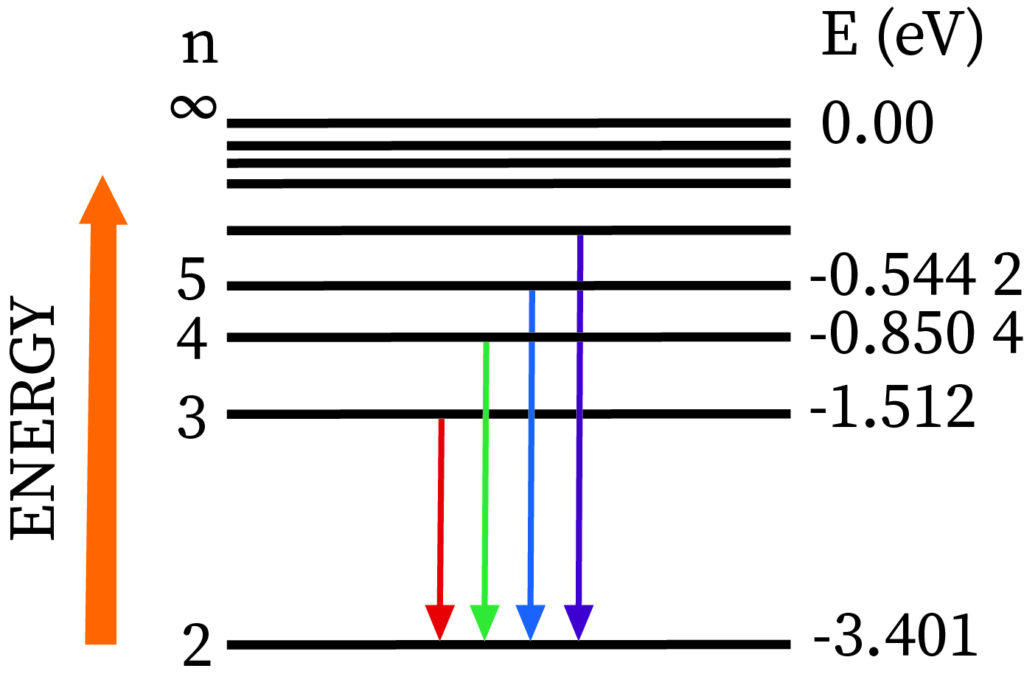
\includegraphics[]{Balmer-Series.jpg}
    \caption{\textbf{Balmer series of Hydrogen}}
    \label{fig:1}
\end{figure}